\section{Выводы по главе}

В главе были рассмотрены общие принципы решений, необходимых ля успешного изменения архитектуры Информатикс, 
была объяснена необходимость проведённых изменений, 
а так обоснованы реализованные решения.
Также в главе был представлен план по изменению архитектуры,
от разворачивания основных сервисов и до пошагового их встраивания.

Были разработаны и внедрены следующие системы и сервисы:
\begin{itemize}
    \item Rmatics;
    \item Rmatics-submit-workers;
    \item Ejudge-listener;
    \item Ejudge-listener-workers;
    \item Система кэшей.
\end{itemize}

\begin{figure}
  \centering
  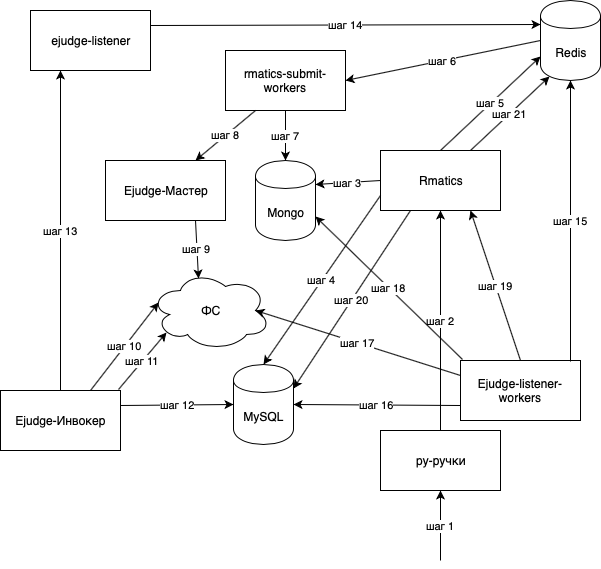
\includegraphics[width=\textwidth]{figures/send_submission.png}
  \caption{Пошаговые взаимодействия сервисов при отправке посылки пользователем}
  \label{fig:send_submission}
\end{figure}

На иллюстрации \ref{fig:send_submission} представлены шаги, которые выполняется при отправке посылки пользователем:

\begin{itemize}
    \item На шаге 1 запрос пользователя с посылкой попадает в py-ручки.
    \item На шаге 2 py-ручка направляет запрос пользователя в сервис Ramtics.
    \item На шаге 3 сервис Rmatics сохраняет исходник посылки в MongoDB.
    \item На шаге 4 сервис Rmatics сохраняет данные о посылке в MySQL.
    \item На шаге 5 сервис Rmatics отправляет в Redis задачу для Rmatics-submit-workers.
    \item На шаге 6 Rmatics-submit-workers получают задачу из Redis.
    \item На шаге 7 Rmatics-submit-workers забирают исходник посылки из MongoDB.
    \item На шаге 8 Rmatics-submit-workers отправляют посылку в Ejudge.
    \item На шаге 9 Ejudge-Мастер сохраняет посылку на ФС.
    \item На шаге 10 Ejudge-Инвокер берёт посылку из ФС.
    \item На шаге 11 Ejudge-Инвокер кладёт протокол и результат тестирования на ФС.
    \item На шаге 12 Ejudge-Инвокер обновляет посылку в БД.
    \item На шаге 13 Ejudge-Инвокер отправляет в Ejudge-listener сообщение о том, что посылка протестирована.
    \item На шаге 14 Ejudge-listener отправляет в Redis задачу на обновление посылки.
    \item На шаге 15 Ejudge-listener-workers получают задачу из Redis.
    \item На шаге 16 Ejudge-listener-workers забирают информацию о посылки из MySQL.
    \item На шаге 17 Ejudge-listener-workers забирают информацию о протоколе и результате тестирования из ФС.
    \item На шаге 18 Ejudge-listener-workers сохраняют информацию о протоколе и результатах тестирования на ФС.
    \item На шаге 19 Ejudge-listener-workers отправляют информацию об обновлённой посылке в Rmatics.
    \item На шаге 20 Rmatics запрашивает из MySQL данные о кэшах, которые после обновления посылки перестали быть валидными.
    \item На шаге 21 Rmatics удаляет из Redis устаревшие кэши.
\end{itemize}

План встраивания сервисов в архитектуру был организован пошагово для того,
чтобы протестировать различные сервисы под реальной нагрузкой,
а так же приобрести уверенность в том, что разработанные решения работают верно.

Такой план дал возможность внедрить новые решения при практически полной доступности Информатикс для пользователей.
